\section{Experimentos e resultados} 

Dado que o sistema de planejamento é geral, foram feitos dois experimentos usando ambos algoritmos: para o mundo dos blocos (subseção~\ref{subsec:expblocos}) e para o mundo dos satélites (subseção~\ref{subsec:expsatelites}). Os dados de entrada são os proporcionados na página no curso (ver \cite{LabIA15}). Para todas as figuras, uma linha vermelha é para o algoritmo Blackbox e uma linha azul para o algoritmo SAT-Plan.

\subsection{Experimentos com mundo dos blocos}
\label{subsec:expblocos}
	A figura~\ref{fig:blockssize} mostra os tamanhos do plano de solução do sistema de planejamento para os problemas proporcionados (com 4 a 8 blocos) e mostra que enquanto o número de blocos aumenta, o tamanho do plano não muda muito. Além, para ambos algoritmos, o plano de solução é igual (por isso, só se ve a linha vermelha).
		\begin{figure}[H]
			\centering
			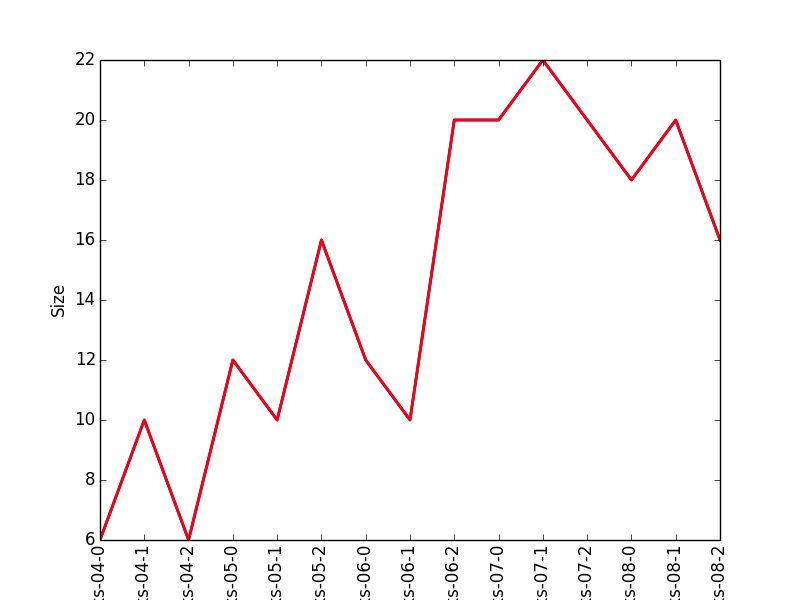
\includegraphics[height=8cm]{images/blocks_size}
			\caption{Tamanhos do plano de solução}
			\label{fig:blockssize}
		\end{figure}
	Mas na figura~\ref{fig:blockstime} se poder ver que os tempos de execução aumentam consideravelmente enquanto o número de blocos aumenta desde segundos até mais de uma hora para 8 blocos em caso de SAT-Plan. No caso de Blackbox os tempos são muito pequenos comparados com SAT-Plan para todos os casos.
		\begin{figure}[H]
			\centering
			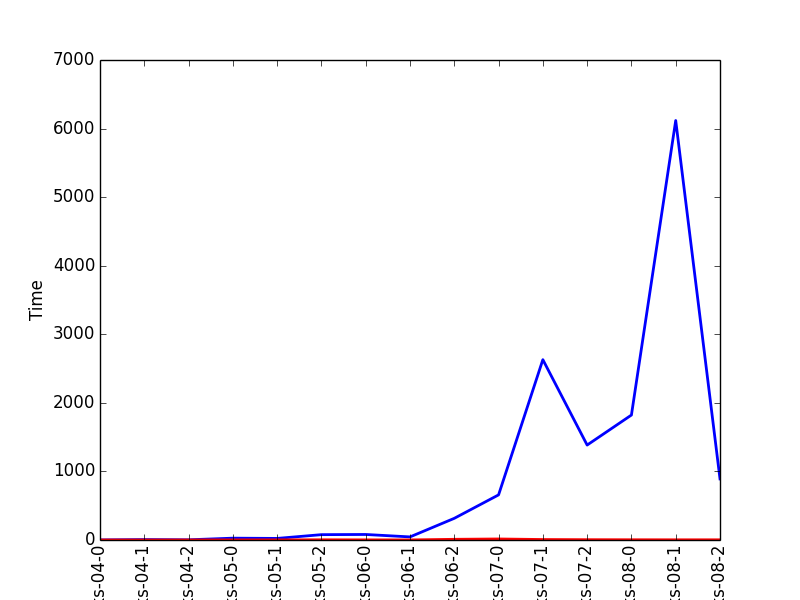
\includegraphics[height=8cm]{images/blocks_time}
			\caption{Tempo de execução (segundos)}
			\label{fig:blockstime}
		\end{figure}
	Além disso, o número de proposições necessárias para solucionar o problema sempre aumenta apesar que o tamanho do plano não muda muito para ambos algoritmos. Mas para o algoritmo Blackbox (linha vermelha) não são necessárias muitas proposições, isto devido a que não coloca as cláusulas de fluentes, se não só de ações e isto adiciona menos proposições comparado com SAT-Plan.
		\begin{figure}[H]
			\centering
			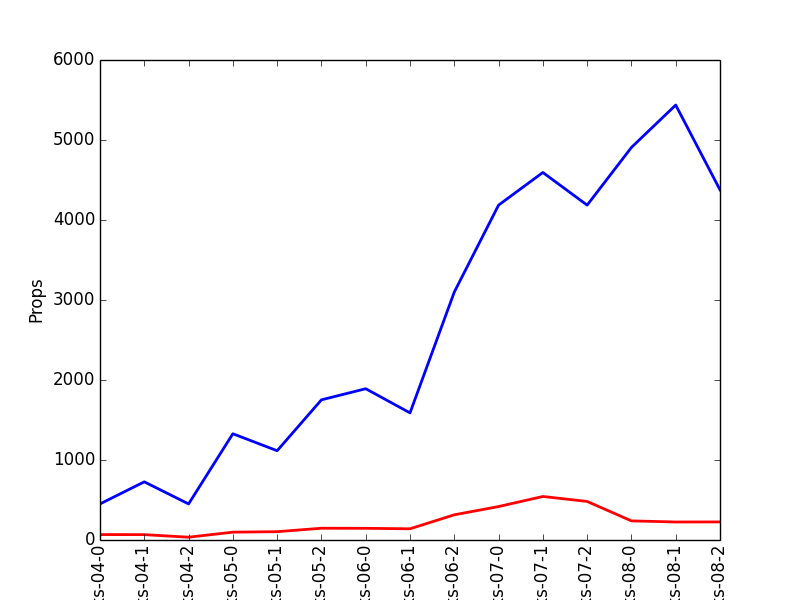
\includegraphics[height=8cm]{images/blocks_props}
			\caption{Número de proposições}
			\label{fig:blocksprops}
		\end{figure}
	Por último, o número de cláusulas aumenta exponencialmente devido que se tem mais variáveis e portanto mais valores para evaluar as ações e fluentes, o que também adiciona mais axiomas em cada iteração dos algoritmos. Mas para o algoritmo Blackbox, o número de cláusulas é consideravelmente menor comparado com SAT-Plan pela mesma razão de número de proposições.
		\begin{figure}[H]
			\centering
			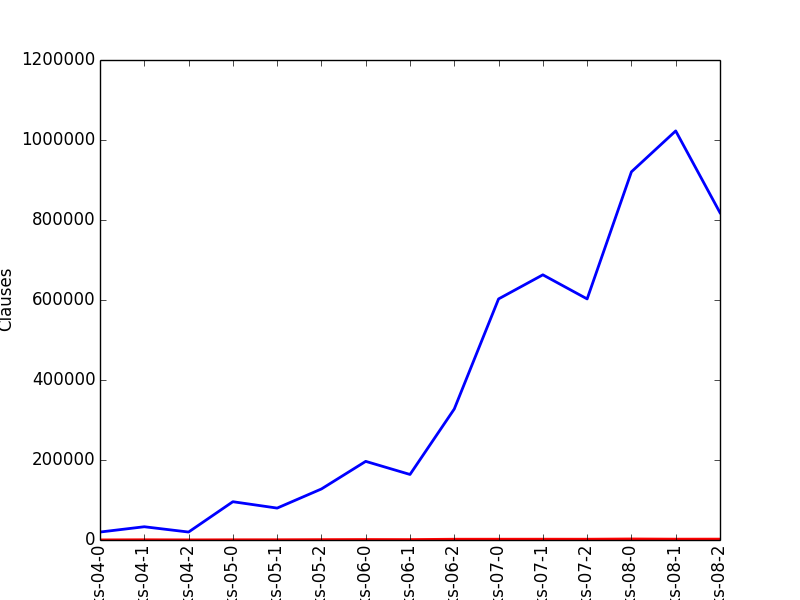
\includegraphics[height=8cm]{images/blocks_clauses}
			\caption{Número de cláusulas}
			\label{fig:blocksclauses}
		\end{figure}
		
\subsection{Experimentos com mundo dos satelites}
\label{subsec:expsatelites}
	A figura~\ref{fig:satsize} mostra os tamanhos do plano de solução do sistema de planejamento para o mundos dos satélites com ambos algoritmos, se pode ver que o tamanho do plano não tem uma relação direta com o número de variáveis e também que ambos algoritmos tem o mesmo tamanho de plano de solução para os problemas.
		\begin{figure}[H]
			\centering
			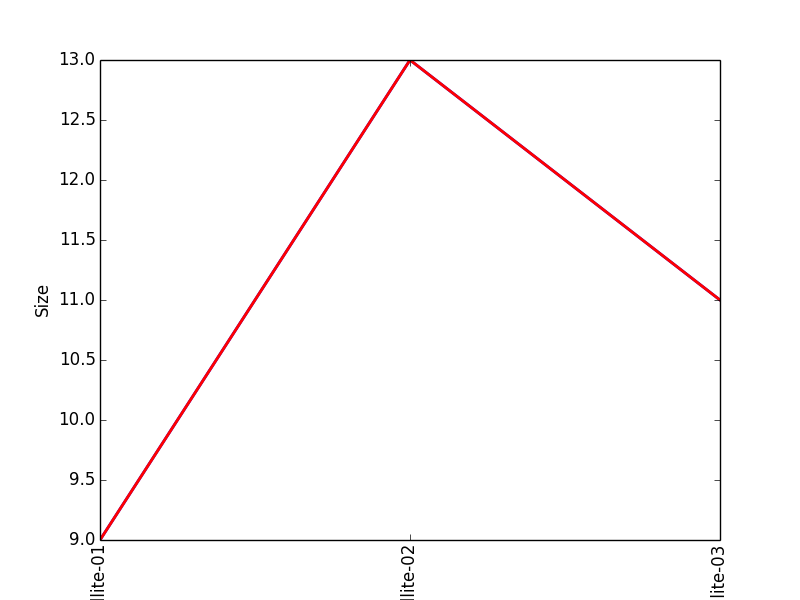
\includegraphics[height=8cm]{images/satellite_size}
			\caption{Tamanhos do plano de solução}
			\label{fig:satsize}
		\end{figure}
	Mas na figura~\ref{fig:sattime} se poder ver que os tempos de execução aumentam consideravelmente enquanto o número de variáveis aumenta. Como na subseção~\ref{subsec:expblocos} aqui também tem tempos de execução consideravelmente baixos comparados com SAT-Plan.
		\begin{figure}[H]
			\centering
			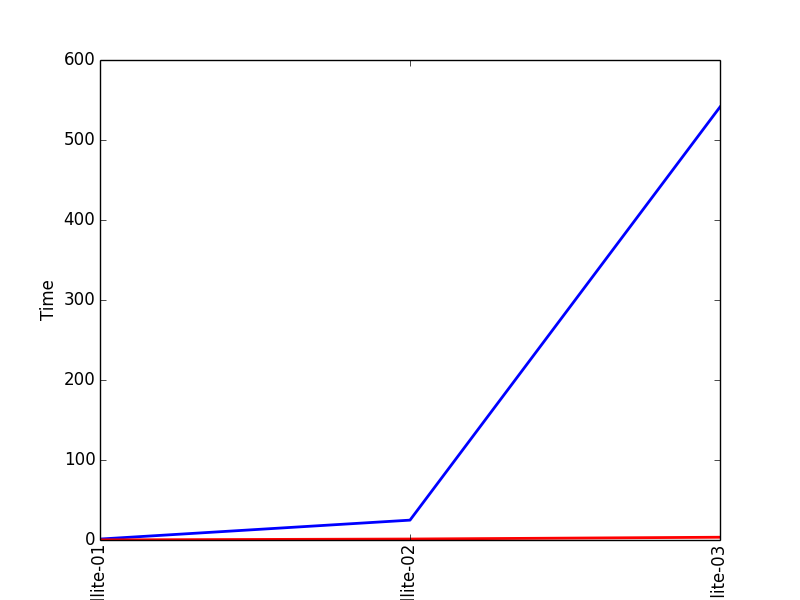
\includegraphics[height=8cm]{images/satellite_time}
			\caption{Tempo de execução (segundos)}
			\label{fig:sattime}
		\end{figure}
	Além disso, o número de proposições aumenta muito em cada incremento de número de variáveis para SAT-Plan, mas não muda muito para Blackbox.
		\begin{figure}[H]
			\centering
			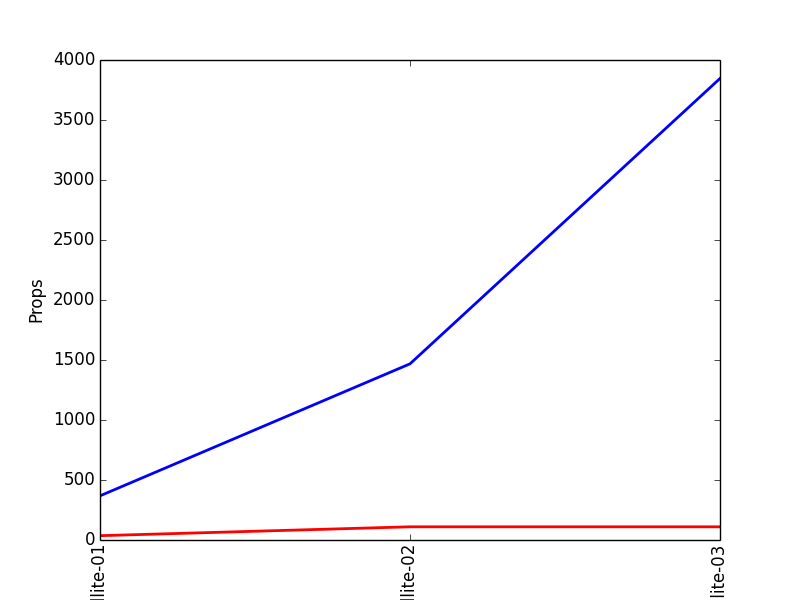
\includegraphics[height=8cm]{images/satellite_props}
			\caption{Número de proposições}
			\label{fig:satprops}
		\end{figure}
	Por último, são necessárias mais de dois milhões de cláusulas para solucionar o tercer archivo de dados de entrada com SAT-Plan e menos de dois mil para Blackbox.
		\begin{figure}[H]
			\centering
			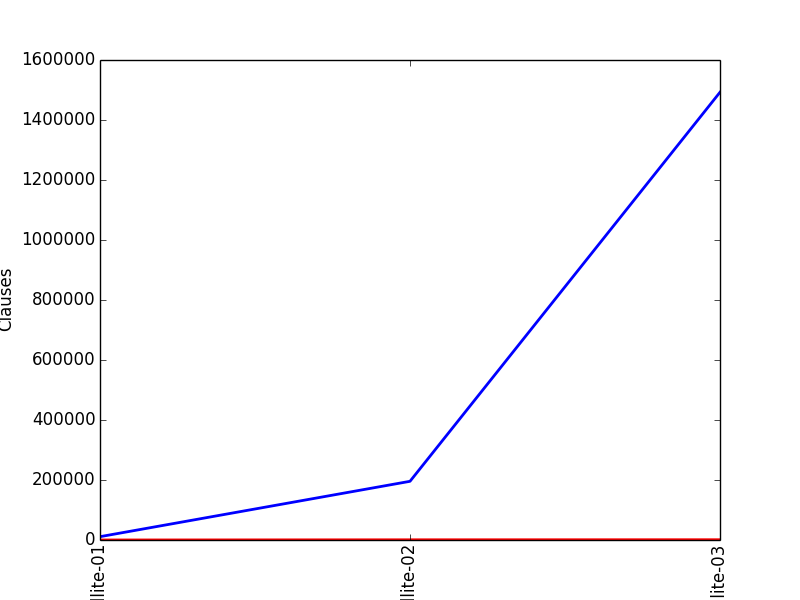
\includegraphics[height=8cm]{images/satellite_clauses}
			\caption{Número de cláusulas}
			\label{fig:satclauses}
		\end{figure}
\newpage